\documentclass[12pt, openany]{report}
\usepackage[utf8]{inputenc}
\usepackage[T1]{fontenc}
\usepackage{amsmath,amsfonts,amssymb}
\usepackage{amssymb}
\usepackage{multicol}
\usepackage[a4paper,left=2.5cm,right=2.5cm,top=2.5cm,bottom=2.5cm]{geometry}
\usepackage[english]{babel}
\usepackage{libertine}
\usepackage{graphicx}
\usepackage{wrapfig}
\usepackage{float}
\usepackage{nicematrix}
\usepackage{enumitem}
\usepackage{amsthm}
\usepackage{pythonhighlight}
\usepackage[]{titletoc}
\usepackage{empheq}
\usepackage{titlesec}
\usepackage{mathpazo}
\usepackage{xfrac}
\usepackage{textcomp}
\usepackage{mathtools}
\usepackage{caption}
\usepackage{tabularray}
\usepackage{subcaption}
\usepackage[bottom]{footmisc}
\usepackage{pdfpages}
\usepackage{tabularx}
\usepackage[skins]{tcolorbox}

\theoremstyle{definition}
\newtheorem{thm}{Theorem}[chapter]
\newtheorem{definition}[thm]{Definition}
\newtheorem{exmp}[thm]{Example} 
\newtheorem{lem}[thm]{Lemma}
\newtheorem{crl}[thm]{Corollary}

\titleformat{\chapter}[display]
  {\normalfont\bfseries}{}{0pt}{\Huge}
\usepackage{hyperref}
\newcommand{\hsp}{\hspace{20pt}}
\newcommand{\HRule}{\rule{\linewidth}{0.5mm}}
\newcommand\independent{\protect\mathpalette{\protect\independenT}{\perp}}
\def\independenT#1#2{\mathrel{\rlap{$#1#2$}\mkern2mu{#1#2}}}

% Define a new tcolorbox style with a red border and transparent interior
\tcbset{
    redbox/.style={
        enhanced,
        colframe=red,
        colback=white,
        boxrule=1pt,
        sharp corners,
        before skip=10pt,
        after skip=10pt,
        box align=center,
        width=\linewidth-2pt, % Adjust the width dynamically
    }
}
\newcommand{\boxedeq}[1]{
\begin{tcolorbox}[redbox]
    \begin{align}
        #1
    \end{align}
\end{tcolorbox}
}
\newcommand{\R}{\mathbb{R}}
\newcommand{\C}{\mathbb{C}}
\begin{document}


\begin{titlepage}
    \begin{sffamily}
    \begin{center}
        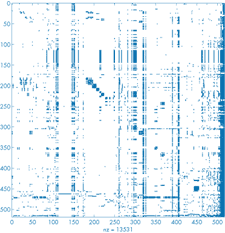
\includegraphics[scale=1]{img/page_de_garde.png} \\[1cm]
        \HRule \\[0.4cm]
        { \huge \bfseries LINMA2380 Matrix Computations \\[0.4cm] }
    
        \HRule \\[1.5cm]
        \textsc{\LARGE Simon Desmidt}\\[1cm]
        \vfill
        \vspace{2cm}
        {\large Academic year 2024-2025 - Q1}
        \vspace{0.4cm}
         
        
\includegraphics[width=0.15\textwidth]{img/epl.png}
        
        UCLouvain\\
    
    \end{center}
    \end{sffamily}
\end{titlepage}

\setcounter{tocdepth}{1}
\tableofcontents
\chapter{Reminders}
\section{Algebraic structures}
\begin{itemize}
    \item A semigroupe is a set together with an associative binary operation \((E,+)\).
    \item A monoid is a semigroup with a neutral element.
    \item A group is a monoid in which every element has an inverse.
    \item A commutative group is a group whose binary operation is commutative.
    \item A ring is a triple \((E,+,\cdot)\) such that
    \begin{itemize}
        \item [\(\bullet\)] \((E,+)\) is a commutative group;
        \item [\(\bullet\)] \((E,\cdot)\) is a monoid;
        \item [\(\bullet\)] $\cdot$ is distirbutive with respect to \(+\).
    \end{itemize}
    \item An integral domain is a commutative ring in which the product of any two nonzero elements in nonzero : \[\forall x,y\in E, x,y\neq 0\qquad xy\neq 0\]. This implies that the equation \(ax=b\) with \(a\neq 0\) has at most one solution. 
    \item An Euclidean domain is an integral domain such that for every two elements in the domain, we can perform the Euclidean division: \[\forall (a_1,a_2), \quad \exists (q,r) : \quad a_1=a_2q+r \text{ with }r<a_2\]
    \item A field is a commutative ring \((E,+,\cdot)\) such that every \(a\in E\setminus \{0\}\) has a multiplicative inverse.
    \item \((K,E,+)\) is a module over the ring \((K,+,\cdot)\) if 
    \begin{itemize}
        \item [\(\bullet\)] \((E,+)\) is a commutative group;
        \item [\(\bullet\)] the external composition operation \(\cdot:K\times E\rightarrow E\) satisfies 
        \begin{itemize}
            \item \((a+b)\cdot x = a\cdot x+b \cdot x \qquad a\cdot (x+y) = a\cdot x+a\cdot y\)
            \item \(a\cdot (b\cdot x) = (a\cdot b)\cdot x\)
            \item \(1\cdot x = x\)
        \end{itemize}
    \end{itemize}
    \item If, in addition to that, \((K,\cdot,+)\) is a field, then \((K,E,+)\) is a vector space over \((K,+,\cdot)\).
    \item \((K,E,+,\cdot)\) is an algebra if 
    \begin{itemize}
        \item [\(\bullet\)] \((K,E,+)\) is a module or a vector space;
        \item [\(\bullet\)] the internal composition operation \(\cdot:E\times E\rightarrow E\) is bilinear.
    \end{itemize}
\end{itemize}
\section{Matrix algebras}
\subsection{Product}
Apart from the usual sum and product of two matrices, we can define the Hadamard and Kronecker products :
\begin{itemize}
    \item Hadamard : \[A_{m\times n}\odot B_{m\times n} \coloneqq [a_{ij}\cdot b_{ij}]_{i,j=1}^{m,n}\]
    \item Kronecker : \[A \otimes B \coloneqq \begin{bmatrix}
        a_{11}B & \dots & a_{1n}B\\
        \vdots & \ddots & \vdots \\
        a_{m1}B & \dots & a_{mn}B\\
    \end{bmatrix}\]
\end{itemize}
A square matrix \(A\in \mathbb{C}^{n\times n}\) is said normal if \(AA^* = A^*\). In the real case, it is said to be orthogonal and \(*\) is equivalent to the transpose. Furthermore, it is said to be unitary if it satisfies the relations \(AA^* = I_n = A^*A\). 
\subsection{Determinant}
We define the quasi-diagonals of a matrix as the \(n\)-tuples of elements of a matrix \(A\), \(a_{1j_1,2j_2,\dots,nj_n}\) where the indices \(\textbf{j} = (j_1,\dots,j_n)\) constitute a permutation of the set \(\{1,2,\dots,n\}\). Thus a quasi-diagonal consists of \(n\) elements of the matrix \(A\) in such a way that no two of them lie in the same row or column of \(A\). For each quasi-diagonal, we define the parity \(t(\textbf{j})\). It is the number of inversions \(j_k>j_p\) for \(k<p\) in \(\textbf{j}\).
\begin{itemize}
    \item With the notation above, we define the determinant of a square matrix \(A_{n\times n}\) as \[\det (A) = \sum_\textbf{j} (-1)^{t(\textbf{j})} a_{1j_1}\cdot a_{2j_2}\cdot \dots \cdot a_{nj_n}\]
\end{itemize}
The determinant has the following properties :
\begin{itemize}
    \item The determinant is multilinear in the rows of \(A\) : \[\det \begin{bmatrix}
        a_{1:}\\ \vdots \\ b_{k:} +\lambda c_{k:} \\ \vdots \\ a_{n:}
    \end{bmatrix} = \det \begin{bmatrix}
        a_{1:}\\ \vdots \\ b_{k:} \\ \vdots \\ a_{n:}
    \end{bmatrix} + \det \begin{bmatrix}
        a_{1:}\\ \vdots \\ \lambda c_{k:} \\ \vdots \\ a_{n:}
    \end{bmatrix}\]
    \item The determinant is alternating in the rows of \(A\) : for \(i\neq j\), \(a_{i:}=a_{j:} \Longrightarrow \det(A) = 0\)
    \item \(\det(I_n) = 1\), where \(I_n\) is the identity matrix.
\end{itemize}
\begin{minipage}{.5\textwidth}
\begin{itemize}
    \item \(\det\begin{bmatrix}
        a_{1:} \\ \vdots \\ a_{i:} \\ \vdots \\ a_{j:} \\ \vdots \\ a_{n:}
    \end{bmatrix} = - \det\begin{bmatrix}
        a_{1:} \\ \vdots \\ a_{j:} \\ \vdots \\ a_{i:} \\ \vdots \\ a_{n:}
    \end{bmatrix}\)
\end{itemize}
\end{minipage}
\begin{minipage}{.5\textwidth}
\begin{itemize}
    \item \(\det\begin{bmatrix}
        a_{1:} \\ \vdots \\ a_{i:} +\lambda a_{j:}\\ \vdots \\ a_{n:}
    \end{bmatrix} = \det\begin{bmatrix}
        a_{1:} \\ \vdots \\ a_{i:} \\ \vdots \\ a_{n:}
    \end{bmatrix}\)
\end{itemize}
\end{minipage}
\begin{itemize}
    \item \(\det (\lambda A)=\lambda^n \det(A)\)
    \item for \(i\neq j\), \(a_{i:} = \lambda a_{j:} \Longrightarrow \det(A) = 0\)
    \item \(\det(A^T) = \det(A)\)
    \item \(\det(A^*) = \overline{\det(A)}\), if \(A\in \mathbb{C}^{n\times n}\)
    \item [\(\rightarrow\)] N.B.: any property of the determinant established for the rows of matrices also holds for the columns.
    \item The minor \(A_{(kl)}\) of dimension \(n-1\) of a matrix \(A_{n\times 
 n}\) is the determinant of the submatrix obtained by removing the \(k\)the row and the \(l\)th column. From this, we can note the determinant as a linear combination of the elements of a row or column : \[\det(A) = a_{1j}A_{1j}^c + a_{2j}A_{2j}^c + \dots + a_{nj}A_{nj}^c \\ \det(A) = a_{i1}A_{i1}^c + a_{i2}A_{i2}^c + \dots + a_{in}A_{in}^c\] where the coefficient \(A_{kl}^c\) is called the cofactors of the corresponding element \(a_{kl}\)\footnote{\(A_{kl}^c = (-1)^{k+l}A_{(kl)}\).}
\end{itemize}
\subsubsection{Laplace and Binet-Cauchy relations}
For the pairs of \(p\)-tuples \[\textbf{i}_p \coloneqq (i_1,\dots,i_p)\text{ and }\textbf{j}_p\coloneqq (j_1,\dots j_p)\] satisfying \[1\le i_1<\dots<i_p\le n\text{ and } 1\le j_1<\dots<j_p\le n\] we define the minors of order \(p\) of \(A\) as 
\begin{equation}
    A\begin{pmatrix}
        \textbf{i}_p\\ \textbf{j}_p
    \end{pmatrix} \coloneqq \det[a_{i_k,j_l}]_{k,l=1}^p
\end{equation}
We also define the complementary cofactors of \(A\) as 
\begin{equation}
    A^c\begin{pmatrix}
        \textbf{i}_p\\ \textbf{j}_p
    \end{pmatrix} \coloneqq (-1)^s A\begin{pmatrix}
        \textbf{i}_p^c\\ \textbf{j}_p^c
    \end{pmatrix}
\end{equation}
where \(s = \sum_{k=1}^p(i_k+j_k)\) and \(\textbf{i}_p^c\) is the set complement of \(\textbf{i}_p\) (same for \(\textbf{j}_p\)). \\
\underline{Laplace Theorem:}\\
Let \(A\) ne a matrix of dimensions \(n\times n\) and \(\textbf{i}_p\) be a \(p\)-tuple of rows (and \(\textbf{j}_p\) for the columns). Then, \(\det(A)\) is equal to the sum of the products of all possibles minors located in these rows/columns with their complementary cofactors:
\begin{equation}
    \begin{cases}
        \det(A) = \sum_{\textbf{j}_p}A\begin{pmatrix}
            \textbf{i}_p\\\textbf{j}_p
        \end{pmatrix} A^c\begin{pmatrix}
            \textbf{i}_p\\\textbf{j}_p
        \end{pmatrix}\\
        \det(A) = \sum_{\textbf{i}_p}A\begin{pmatrix}
            \textbf{i}_p\\\textbf{j}_p
        \end{pmatrix} A^c\begin{pmatrix}
            \textbf{i}_p\\\textbf{j}_p
        \end{pmatrix}\\
    \end{cases}
\end{equation}
\underline{Binet-Cauchy Theorem:}\\
Let \(\textbf{m}\) be the \(m\)-tuple \((1,\dots,m)\). Let \(A\) and \(B\) be matrices of dimensions \(m\times n\) and \(n\times m\) respectively. If \(m\le n\), then 
\begin{equation}
    \det(AB) = \sum_{\textbf{j}_m} = A\begin{pmatrix}
        \textbf{m}\\ \textbf{j}_m
    \end{pmatrix} B\begin{pmatrix}
        \textbf{j}_m\\ \textbf{m}
    \end{pmatrix}
\end{equation}
\subsection{Inverse and rank}
\begin{itemize}
    \item The adjugate matrix of a square matrix \(A_{n\times n}\) is defined as \[adj(A) \coloneqq [A_{ji}^c]_{i,j=1}^n\]
\end{itemize}
Then, for every square matrix \(A_{n\times n}\), we have
\begin{equation}
    A\cdot adj(A) = \det(A) I_n = adj(A)\cdot A
\end{equation}
Every matrix \(A_{m\times n}\) whose elements belong to a field \(\mathcal{F}\) can be brought to the following form by means of invertible (or elementary) transformations of rows and columns:
\begin{equation}
    RAQ = \begin{pNiceArray}{cc|c}
    I_r && 0_{r\times (n-r)}\\
  \hline
  0_{(m-r)\times r} && 0_{(m-r)\times (n-r)}\\
\end{pNiceArray}
\end{equation}
The rank of a matrix \(A_{m\times n}\) whose elements belong to a field \(\mathcal{F}\) is equal to the largest size of its nonzero minors. As a corollary, any non-singular matrix whose elements belong to a field \(\mathcal{F}\) can be written as a product of elementary transformations.\\

\underline{Schur complement:}\\
Let \(A_{n\times n}\) be an invertible submatrix of the matrix \[M_{(n+p)\times (n+m)} = \begin{pmatrix}
    A & B\\ C & D\\
\end{pmatrix}\]
Then the rank of \(M\) satisfies 
\begin{equation}
    rank(M) = n + rank(D-CA^{-1}B)
\end{equation}
And the matrix \(D-CA^{-1}B\) is called the Schur complement of \(M\). 
\chapter{QR form}
TODO
\chapter{Unitary transformations and SVD}
\section{Introduction and definitions}
\begin{itemize}
    \item A unitary matrix is a matrix \(U\in \C^{n\times n}\) such that \(U^*U=I\), i.e. its column are orthogonal.
    \item An isometry is a matrix \(U\in \C^{m\times n}\), \(m\neq n\), such that \(U^*U=I\). We have \(\lVert Ux\rVert =\lVert x \rVert\). 
\end{itemize}
\section{Diagonalization by unitary transformations}
The goal here is to have a matrix decomposition of the form 
\begin{equation}
    A = R\begin{pmatrix}
        I_r & 0\\ 0& 0 \\
    \end{pmatrix}Q^{-1}
\end{equation}
for any arbitrary matrix \(A_{m\times n}\), and with \(R,Q\) being unitary (if \(A\) is complex) or orthogonal (if \(A\) is real). We limit ourselves here to transformation matrices that are isometries\footnote{To define.}. This means that the invariants that we obtain characterize the way the matrix act on the norm of vectors. 
\begin{thm}
    Every Hermitian\footnote{\(A=A^*\)} matrix \(A\in \C^{n\times n}\) can be diagonalized by a unitary transformation \(U\in \C^{n\times n}\):
    \begin{equation}
        U^*AU = \begin{pmatrix}
            \lambda_1 & 0 & \dots & 0\\
            0&\ddots &\ddots \vdots \\
            \dots & \ddots & \ddots & 0\\
            0 & \dots & 0 & \lambda_n\\
        \end{pmatrix}
    \end{equation}
    with \(\lambda_i\in \R\).
\end{thm}
\begin{thm} 
    The eigenvalues of a Hermitian matrix \(A\in \C^{n\times n}\) are invariant under unitary similarity transformations:
    \begin{equation}
        B=U^*AU
    \end{equation}
    Every class of equivalence defined by this transformation group has a unique canonical representative which is the diagonal matrix \(\Lambda\) with the eigenvalues of \(A\) decreasing along the diagonal.
\end{thm}
\begin{thm}[\textbf{Singular Value Decomposition}]
    For every matrix \(A\in \C^{m\times n}\), there exist unitary transformations \(U\in \C^{m\times m}\) and \(V\in \C^{n\times n}\) such that 
    \begin{equation}
        A=U\Sigma V^* \qquad \Sigma = \begin{pNiceArray}{ccc|c}
            \sigma_1 &        & 0                  &  \\
                     & \ddots &                    & 0_{r\times (n-r)}\\
            0        &        & \sigma_r           &  \\ \hline
                     & 0_{(m-r)\times r} & & 0_{(m-r)\times (n-r)}\\
          \end{pNiceArray}
        \end{equation}
    with real positive singular values \(\sigma_1\ge \dots \ge \sigma_r > 0\). The value \(r\) and the \(r\)-tuple \((\sigma_1,\dots,\sigma_r)\) are uniquely defined and, as a consequence, the matrix \(\Sigma\) constitutes a canonical form under unitary transformations, i.e. under transformations of the forme \(B = \tilde U^* A\tilde V\). Where \(\tilde U, \tilde V\) are two unitary matrices. 
\end{thm}
\underline{Properties:}
\begin{itemize}
    \item If the matrix \(A\) is real, \(U,V\) are orthogonal matrices;
    \item The transformations \(U,V\) diagonalize the matrices \(AA^*\) and \(A^*A\) respectively, since \(U^*AA^*A = \Sigma \Sigma^T\), \(V^*A^*AV=\Sigma^T\Sigma\), and the columns of \(U,V\) are the eigenvectors of \(AA^*\) and \(A^*A\) respectively.
    \item The transformations \(U,V\) are not uniquely defined. 
\end{itemize}
\end{document}